% Part III — Properties of MoM Estimators
\section{Properties of MoM}

% Slide 9 — MoM Properties
\begin{frame}{Properties of MoM}
  \begin{block}{Summary (formal)}
    Method of moments estimators typically enjoy:
    \begin{itemize}
      \item Consistency (via LLN on sample moments)
      \item Asymptotic normality (via Delta method)
      \item Simplicity in computation
    \end{itemize}
    They are generally not efficient and can be sensitive to outliers.
  \end{block}

  \begin{block}{Intuition / Relevance}
    MoM is attractive when closed-form, quick estimates are needed. In
    applications it is a useful baseline but may be supplanted by MLE when
    efficiency or robustness matter.
  \end{block}

  \vspace{0.7em}
  % Visual moved to a separate frame
\end{frame}

% Visual frame — MoM Properties (visual)
\begin{frame}{Properties of MoM -- Visual}
  \begin{center}
    \begin{adjustbox}{max height=0.40\textheight}
    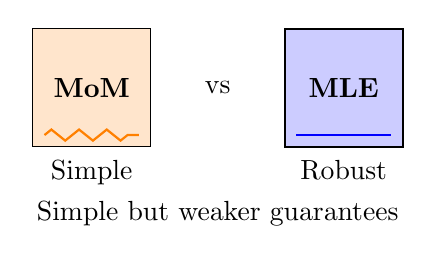
\begin{tikzpicture}[scale=0.8]
      % Simple but weaker structure
      \node[draw, rectangle, fill=orange!20, minimum size=1.5cm] at (-2,0) {\textbf{MoM}};
      \node[below] at (-2, -1) {Simple};

      % vs
      \node at (0, 0) {vs};

      % Solid structure for MLE
      \node[draw, rectangle, fill=blue!20, minimum size=1.5cm, thick] at (2,0) {\textbf{MLE}};
      \node[below] at (2, -1) {Robust};

      % Shaky lines for MoM
      \draw[orange, thick, decorate, decoration={zigzag, amplitude=2pt}] (-2.75, -0.75) -- (-1.25, -0.75);

      % Solid lines for MLE
      \draw[blue, thick] (1.25, -0.75) -- (2.75, -0.75);

      \node at (0, -2) {Simple but weaker guarantees};
    \end{tikzpicture}
    \end{adjustbox}
  \end{center}
\end{frame}